\section{Synthesising Configurations across Multiple Domains}
\label{sec:synth-multi}

In this section, we present an algorithm for 
solving the path-compliance problem in the presence
of multiple domains---i.e., $|\{\Theta(r) \mid r\in V\}|>1$.
However, we assume that the domain splitting $\Theta$ is given to us.
Formally, we are given a set of paths $\Pi$,
a topology $T=(V,L)$,
a domain-assignment function $\Theta$ such that $|\{\Theta(r) \mid r\in V\}|>1$, 
and we want to find functions
$LP$, $W$, and $RF$,  such that
$C=(T,W,RF,LP,\Theta)$ and
$\paths^C(PC) = \Pi$.
We call this problem the \emph{inter-domain synthesis problem}.

\begin{figure*}
	\centering
	\subfloat[Ex1]{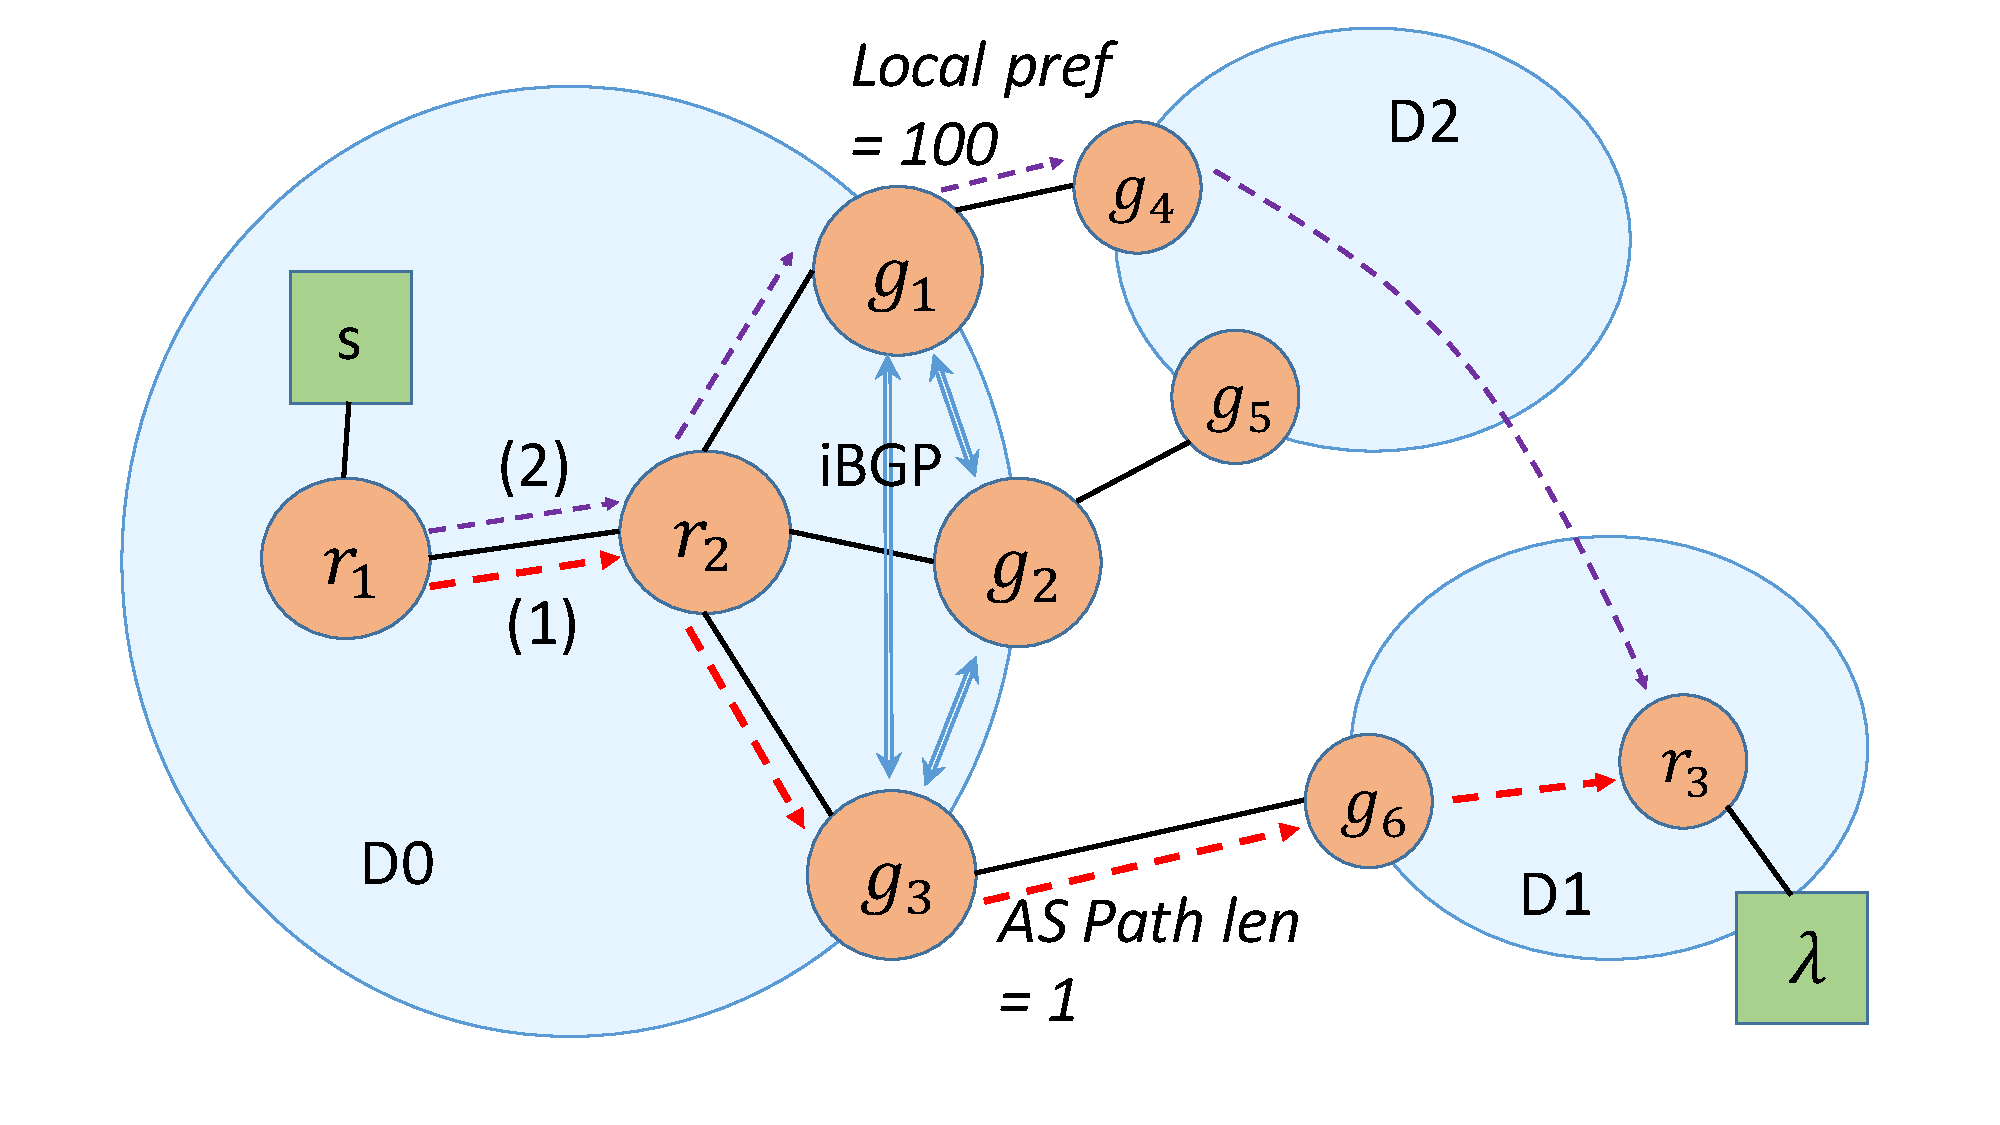
\includegraphics[width=0.66\columnwidth]{figures/bgp-example.pdf}}
	\hfill
	\subfloat[Ex2]{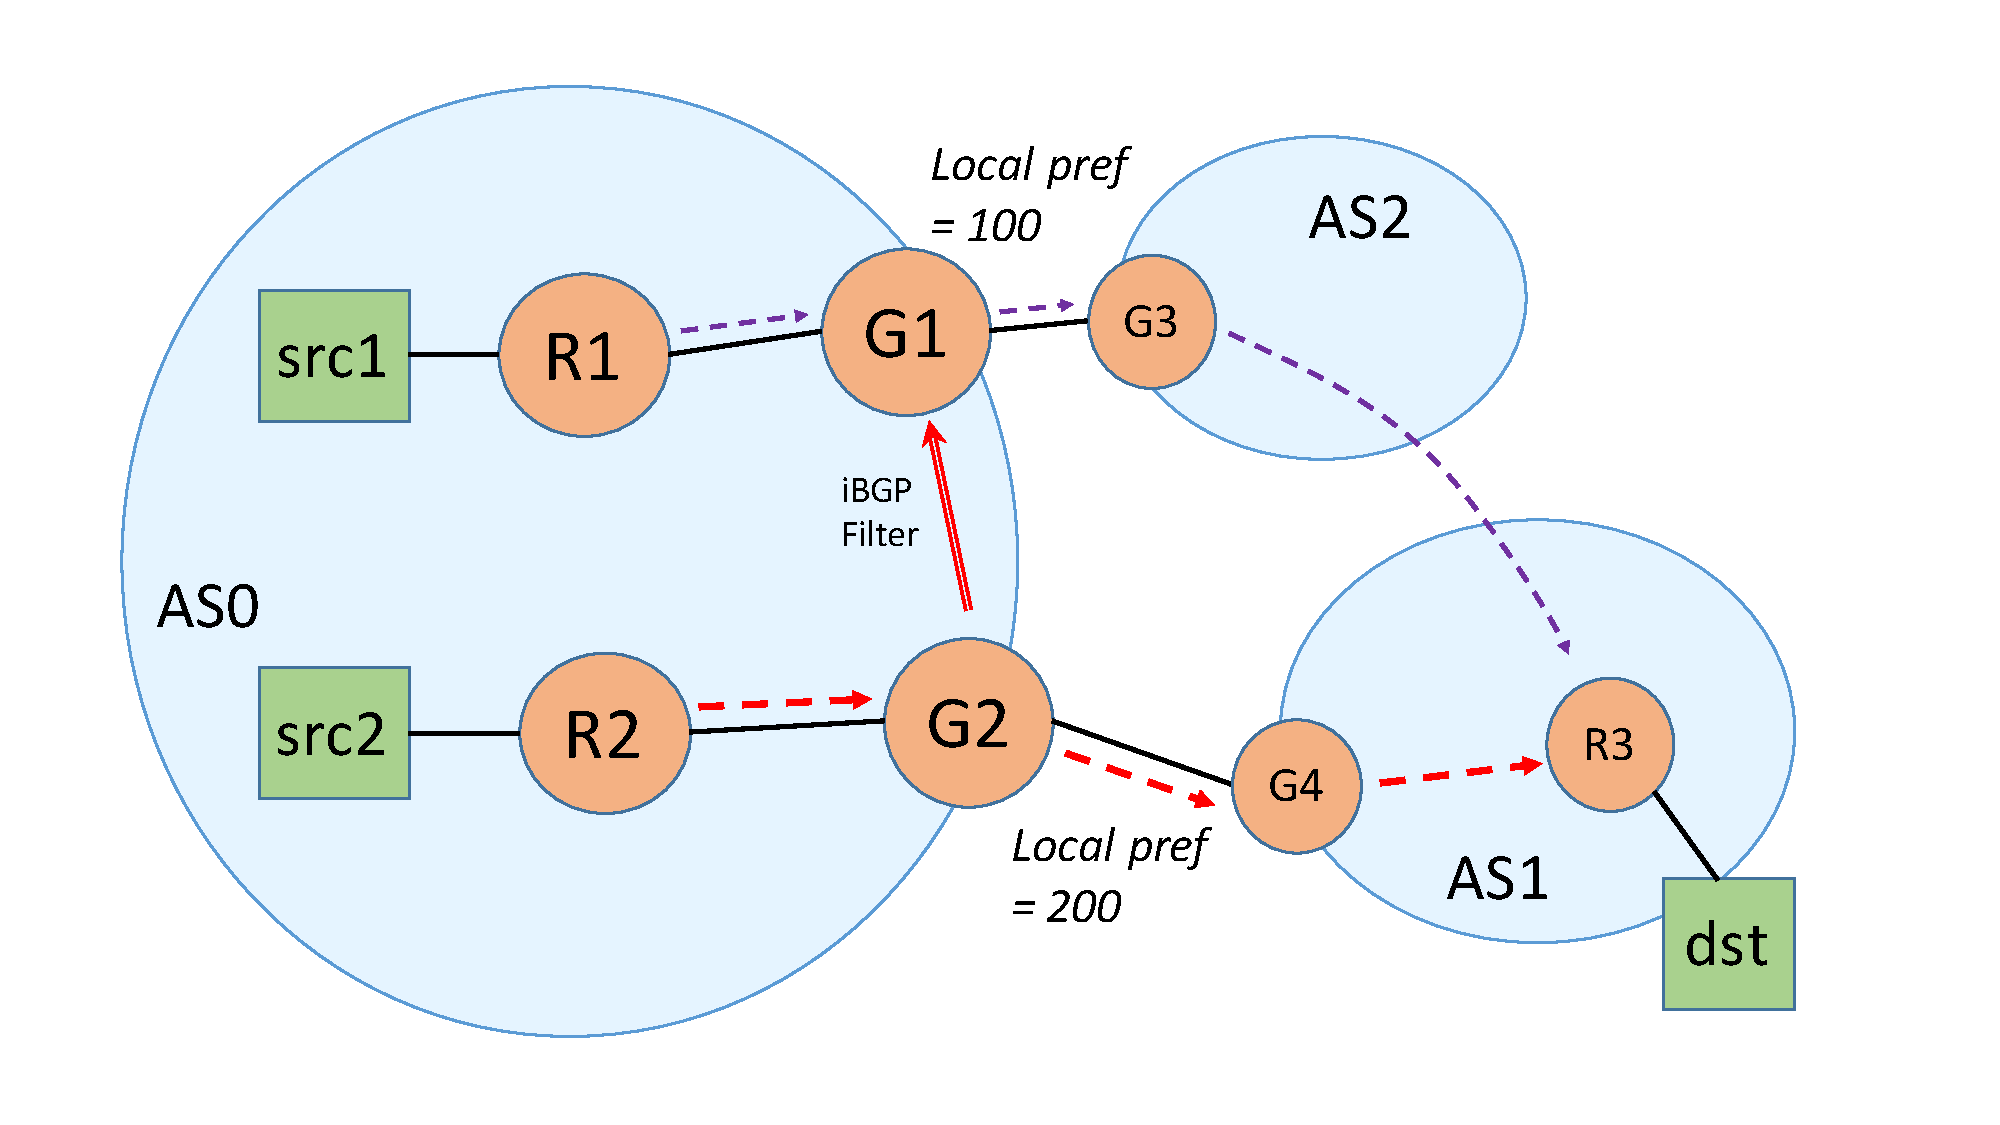
\includegraphics[width=0.6\columnwidth]{figures/bgp-example2.pdf}}
	\hfill
	\subfloat[Ex3]{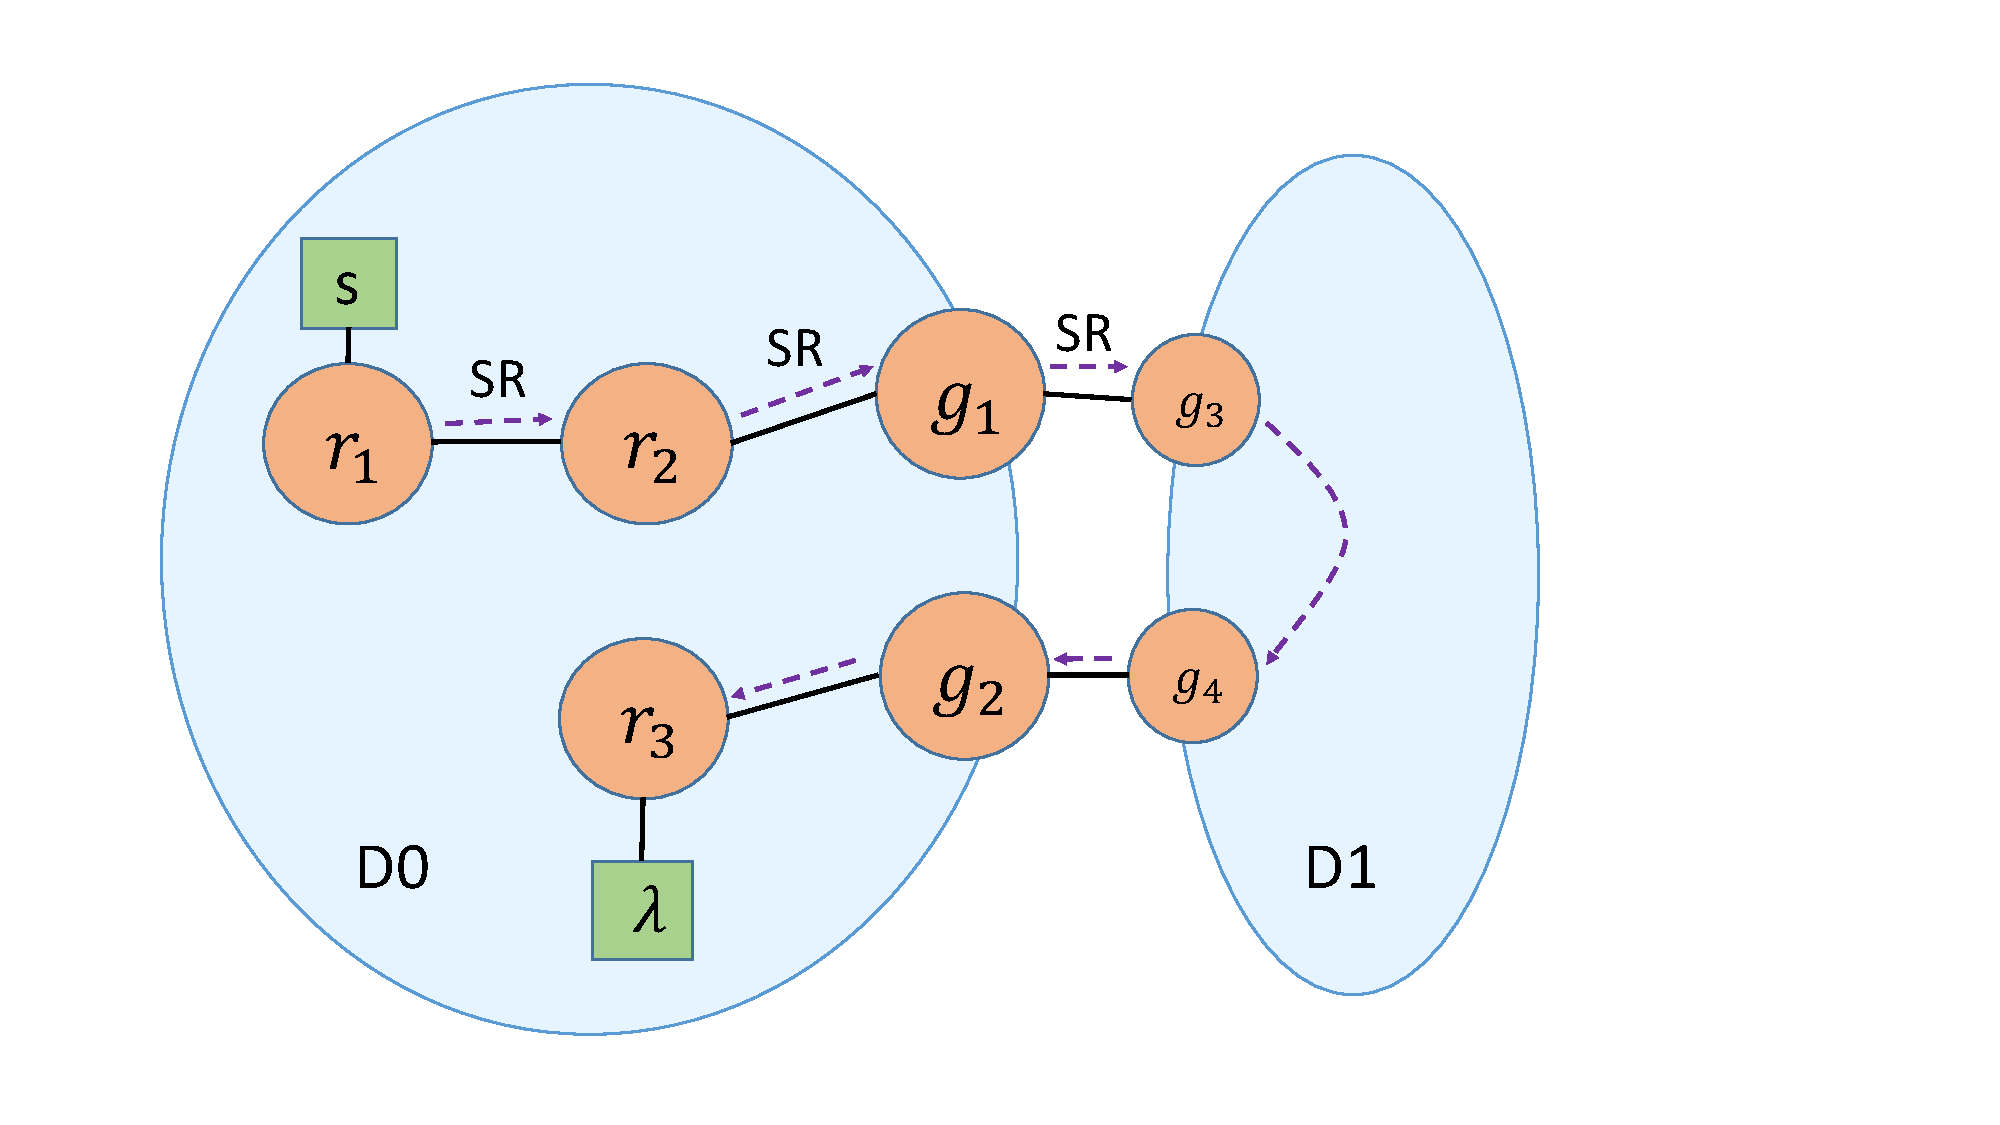
\includegraphics[width=0.5\columnwidth]{figures/static-route.pdf}}
	\compactcaption{\label{fig:bgpexample}
	How to configure inter-domain routing, CHANGE dst to lambda}
\end{figure*}

\subsection{Configuring BGP and Static Routes}
\minisection{BGP}
BGP is a path-vector protocol where each router 
advertises to its peers, 
a route for a destination in the form 
of a path of domains to reach the destination.  
For path-compliance, we need to configure
BGP routers such the route chosen by BGP
and redistributed into OSPF is the policy-compliant
path given as input. We describe three different
cases of how BGP is configured.  

Consider path (1) $\in \Pi$ (\Cref{fig:bgpexample}(a)).
BGP router $g_3$ receives a route $2$ for $\lambda$ with domain path length 1, 
while $g_1$ and $g_2$ will receive routes $1 \rightarrow 2$ 
for $\lambda$ with 
domain path length 2. Since, we need to send traffic along
$g_3$, we do not need to configure any additional BGP variable for $\lambda$,
and the route via $g_3$ is redistributed into domain 0. 
For $\lambda$, the gateway at domain 0 is $g_3$, i.e.,
$G^C(0, r_1, \lambda) = g_3$.

Consider if path (2) $\in \Pi$ to $\lambda$ 
(\Cref{fig:bgpexample}(a)). Since, $g_1$'s route has a longer domain 
path length than $g_3$'s route and equal to $g_2$'s route,
we need to set the local preference of route received by $g_1$ 
(from $g_4$) to 100 (any positive value). Thus, BGP 
will select $g_1$ as the exit gateway for $\lambda$ i.e.,
$G^C(0, r_1, \lambda) = g_1$.

Suppose, the paths for $\lambda$ exited through two different
gateways in a domain (\Cref{fig:bgpexample}(b)).
Path from $r_1$ exits domain 0 through 
gateway router $g_1$, while $r_2$'s traffic exits 
through $g_2$. 
Therefore, both these routes need to be 
redistributed to the OSPF domain. 
Therefore, we assign
$LP(g_1,g_3,\lambda) = 100$ and $LP(g_2,g_4,\lambda) = 200$. For 
router $g_2$ and destination $\lambda$, 
no other route has a local preference value $>200$, thus 
the route along the path is chosen and redistributed into 
OSPF by $g_2$. However at $g_1$, the iBGP route
sent by $g_2$ with local preference 200 will be preferred over
the $g_1\rightarrow g_3$ route which has local preference 100.
Thus, we add a iBGP filter for connection $g_2 \rightarrow g_1$ for
destination IP $\lambda$ ($g_1$ and $g_2$ need not be connected by a 
link directly; iBGP establishes a connection among the 
BGP routers in a domain). Thus, $g_1$ will not receive the
$g_2 \rightarrow g_4$ route from $g_2$, and the route $g_1 \rightarrow
g_3$ route would be chosen as it has the highest local preference
of all routes received by $g_1$, and will be redistributed into the 
OSPF domain. 

\minisection{Static Routes} \label{sec:static}
Consider input path for $\lambda$ 
as shown in \Cref{fig:bgpexample}(c). BGP Gateway $g_1$ 
will receive a advertisement for $\lambda$ with domain
path $(1,0)$ and will reject it because the complete
domain path would have loops $(0,1,0)$. 
Therefore, we require static routes 
to enforce domain paths with loops. For the example in 
\Cref{fig:bgpexample}(c): \\
\hspace*{0.7cm}$SR(r_1,\lambda) = r_2, SR(r_2,\lambda) = g_1, SR(g_1,\lambda) = g_2$ 

\noindent The path from $g_2$ to $\lambda$ does not 
require static routes, as there are no more domain loops.

\minisection{Algorithm}
For a path $\pi = l_1 l_2 \ldots l_m \in \Pi$, we
can divide the path into intra-domain paths and inter-domain
links. We express $\pi$ as 
$\pi_1 idl_1^2 \pi_2 \ldots idl_{n-1}^n \pi_n$ where
each subpath $\pi_i$ is completely in a
domain, i.e., for each 
link $(r_1,r_2) \in \pi_i \implies \Theta(r_1) = \Theta(r_2)$;
and links $idl_1^2, idl_2^3 \ldots idl_{n-1}^n$ 
represent the inter-domain links. The domain path
$\tilde{\pi} = d_1 \ldots d_n$ is the 
domains of the intra-domain path segments in order
: $\forall i \leq n. d_i = \Theta(\pi_i)$ (where
$\Theta(\pi_i)$ denotes the domain of any router in the 
intra-domain path $\pi_i$). 


For a given path $\pi$ and corresponding path $\tilde{\pi}$,
we find the longest non-looped domain subpath ending at
destination domain: $nl = $\texttt{min} $i$ such that
$\forall j \geq i. ~\not\exists k \geq i. d_j = d_k$. 
Therefore, the subpath of $\pi$ corresponding to
domains $d_{nl} \ldots d_n$--- $\pi_{nl} ~idl_{nl}^{nl+1}\ldots idl_{n-1}^n \pi_n$
can be induced by BGP (no loops in the domain path).
For $i \in [1,nl-1]$, all links in $\pi_i$ 
and $l_i^{i+1}$ 
will require a static route for $\lambda$: 
\begin{equation}
\forall (r_1, r_2) \in (\bigcup_{i < nl} \pi_i) \cup (\bigcup_{i < nl} idl_i^{i+1}). ~SR(r_1, \lambda) = r_2
\end{equation}

\noindent 
For each path $\pi$, the intra-domain subpaths which are
not statically routed is aggregated according to the domain 
and \name applies
OSPF synthesis for each domain with the subpaths lying 
in the domain as input. For each destination $\lambda \in \Lambda$, 
BGP is configured accordingly
based on if there is a single gateway in domain (\Cref{fig:bgpexample}(a))
or multiple gateways (\Cref{fig:bgpexample}(b)) for the paths of destination
$\lambda$ in the domain. 



%Static routes have the highest priority and is used to 
%exit and enter a domain multiple times. 
%While static routes
%do not reduce the resilience of the network (all routes are still
%enabled, unlike route-filters), a network under flux will have
%unpredictable routing behaviour, unlike with only OSPF and BGP
%configured at the routers. 
%Also, static routes have to be installed per-destination, thus increasing
%the size of configurations drastically as number of policy paths increase.
%
%Given a path $p$ for subnet $\lambda$ and 
%the corresponding domain path $p_{as}
%= as_1 \rightarrow as_2 \rightarrow \ldots \rightarrow as_m$ (where
%$as_m = \Theta(\lambda)$), static
%routes are required if $p_{as}$ has a domain-loop. 
%To minimize
%the number of static routes, we find 
%the smallest $i \in [1,m]$ 
%such that $\overline{p_{as}} = as_i \rightarrow as_{i+1}
%\rightarrow \ldots \rightarrow as_m$ has no loops. 
%Therefore, $\overline{p_{as}}$ is the longest domain-loop-free
%subpath of $p_{as}$, and be can be enforced using BGP and OSPF. For the 
%network path corresponding to domain path $as_1 \rightarrow as_2 
%\rightarrow \ldots \rightarrow as_{i-1}$, we require static
%routing rules for each next-hop. The static routing score
%is the total number of static route hops required to enforce
%the input paths.
%\todo{Write about the BGP paths are extracted for the next phase}
%
%\subsubsection{BGP Local Preference Entries}
%\name uses BGP local preference to route traffic
%for a particular subnet to the next domain via a specific 
%gateway as per the input paths obtained. 
%As shown in \Cref{} (Refer
%to ex), if there are multiple exit gateways from an domain 
%for a subnet $\lambda$, we require local preference entries at the 
%gateways and iBGP filters among these gateways for $\lambda$.
%
%For a domain $d$ and subnet $\lambda$, consider the set 
%of paths to $\lambda$ exiting $d$ using BGP (and not statically
%routed as described in \Cref{sec:static}). Let $E$ denote the
%set of exit gateway routers for the paths of $\lambda$. 
%If $|E| = 1$, if gateway $g$ receives a route with 
%strictly shortest domain path length (\Cref{alg:bgppathrules}) 
%which enforces the paths
%for $\lambda$, we do not need to configure local preference
%entries on any BGP router in the domain for $\lambda$. If
%the exit route chosen by the gateways for $\lambda$ does not 
%enforce the paths, \name configures a local preference entry
%for $\lambda$ at exit gateway, and thus, the exit route chosen
%by BGP enforces the input paths for $\lambda$ in the domain.
%
%If $|E| ~> 1$, multiple BGP routes must be redistributed to 
%the OSPF domain.
%E local prefs + E(E - 1) iBGP filters!
%
%\todo{Changes to OSPF synthesis to ensure closest gateway}
\subsection{Modified OSPF Synthesis for Multiple Gateways}
When BGP routes of destination $\lambda$ 
are redistributed by multiple gateways to an 
OSPF domain, \name uses a modified OSPF synthesis
algorithm from \secref{sec:ospfsynthesis}. This is 
required because an OSPF router will choose
the closest BGP gateway in terms of OSPF distance 
for $\lambda$. For instance, a router $r$ will choose
from gateways $g_1$ and $g_2$ according to the $r-g_1$
and $r-g_2$ distance. Therefore, given the input path in
the domain $\pi_1=r \rightarrow^+ g_1$, \name adds additional
constraints ensuring the distance to $g_2$ from routers
on the path $\pi_1$ is strictly
greater than the distance to $g_1$. 

Let us define $\Gamma_\lambda$ to be the set of gateway
routers for destination $\lambda$ in the domain. 
$r_1 \rightarrow^+_{\xi_{\lambda}} r_2$ holds if
$r_2$ is reachable from $r_1$ in the destination tree $\xi_\lambda$.
\name adds the following constraints 
to ensure a router
chooses the correct gateway so that input 
paths are induced: 
\begin{multline} \label{eq:gateway}
\forall g \in \Gamma_{\lambda}.~\forall r \in \xi_\lambda 
\wedge r \rightarrow^+_{\xi_{\lambda}} g. \\
~\forall g' \in \Gamma_{\lambda} \wedge g' \not= g. 
~\forall n' \in N(r) \setminus N_{\xi_\lambda}(r). \\
E(r, n') + D(n', g') > \sum_{\mathclap{\substack{(r_i,r_j) \in r \rightarrow^+_{\xi_{\lambda}} g }}} 
E(r_i, r_j) 
\end{multline}
Like unmodified OSPF synthesis, the system of
constraints generated could be inconsistent and require
route-filters to eliminate constraints. In this scenario,
we need to filter shorter routes to gateways which are
not on the input path, and 
thus the synthesized configuration would forward traffic to
the gateway specified by the input path. 
We use the same 
approach of picking route-filters from the IIS
(\secref{sec:routefilter}), route-filter $((r, n'), \lambda)$
maps to following constraint in the IIS for some $g,g'$: 
\begin{equation}
E(r, n') + D(n', g') > \sum_{\mathclap{\substack{(r_i,r_j) \in r \rightarrow^+_{\xi_{\lambda}} g }}} 
E(r_i, r_j) 
\end{equation}